\documentclass[article,shortnames]{jss}

\usepackage{tikz}
\usepackage{attrib}
\Plainauthor{Eric Schulte, Dan Davison, Thomas Dye, Carsten Dominik}
\author{Eric Schulte\\University of New Mexico \And Dan Davison\\University of Oxford and Counsyl \AND Thomas Dye\\University of Hawai`i \AND Carsten Dominik\\University of Amsterdam and Radboud University Nijmegen}
\title{A Multi-Language Computing Environment for Literate Programming and Reproducible Research}
\Shorttitle{Computational Environment for Mixed Prose and Code}
\Keywords{literate programming, reproducible research, compendium, web, emacs}
\Address{Eric Schulte\\Department of Computer Science\\University of New Mexico\\1 University of New Mexico\\Albuquerque, NM 87131\\United States of America\\E-mail: eschulte@cs.unm.edu\\URL: http://cs.unm.edu/$\sim$eschulte/}
\Abstract{We present a new computing environment for authoring mixed natural and computer language documents. In this environment a single hierarchically-organized plain text source file may contain a variety of elements such as code in arbitrary programming languages, raw data, links to external resources, project management data, working notes, and text for publication. Code fragments may be executed in situ with graphical, numerical and textual output captured or linked in the file. Export to \LaTeX{}, \proglang{HTML}, \LaTeX{} \proglang{Beamer}, \proglang{DocBook} and other formats permits working reports, presentations and manuscripts for publication to be generated from the file. In addition, functioning pure code files can be automatically extracted from the file. This environment is implemented as an extension to the Emacs text editor and provides a rich set of features for authoring both prose and code, as well as sophisticated project management capabilities.}

\begin{document}

\section{Introduction}
\label{sec-1}

There are a variety of settings in which it is desirable to mix prose,
code, data, and computational results in a single document.
\begin{itemize}
\item \emph{Scientific research} increasingly involves the use of computational
  tools. Successful communication and verification of research results
  requires that this code is distributed together with results and
  explanatory prose.
\item In \emph{software development} the exchange of ideas is accomplished
  through both code and prose; code provides concrete implementation
  while prose provides higher level explanation.  Without proper
  documentation, the usability and future extensibility of
  computational tools are compromised.
\item In \emph{pedagogical} environments it is important for descriptions of
  algorithms or techniques to go hand-in-hand with
  implementations and example output.  These environments include
  in-class presentations, published books and articles, online
  tutorials, and experiential blogs with accompanying instructions.
\end{itemize}

In each of the situations described above, prose in the absence
of code is typically insufficient.  Similarly, code
without expository prose is a less-than-ideal medium for communication
between people. In this paper we describe the plain text markup
language \pkg{Org-mode}, with a focus on its provision of a unified
environment supporting many different approaches to composition and
application of combined prose and code (Figure \ref{fig:overview}).  Working in
\pkg{Org-mode} is an extension of standard text editing. Thus, trivial usage
of \pkg{Org-mode} is nothing more than text editing, from which point the
user can start to add special plain text \pkg{Org-mode}
elements to the document.  \pkg{Org-mode} is therefore easy to adopt and
aims to be a general solution for authoring projects with mixed
computational and natural languages.  It supports multiple programming languages,
export targets, and work flows.

  \usetikzlibrary{shapes,arrows,shadows,decorations,decorations.text,through}
  \tikzstyle{page} = [rectangle, draw, text width=9em,
  text centered, rounded corners,
  node distance=3cm, minimum height=1em,
  font=\tiny,
  fill=blue!20,
  general shadow={
    fill=black!30,
    shadow xshift=0.16cm,
    shadow yshift=-0.16cm
  },
  very thick,
  draw=blue]
  \begin{figure}[t!]
    \centering
    \begin{tikzpicture}[->,>=stealth', shorten >=1pt, auto, scale=0.65]
      \node [page] (org) at (0,0) {
        \begin{center}
          \normalsize{Org-mode}
        \end{center}
  \begin{verbatim}
    * Plain Text Markup
    - prose composition
    - code composition
    - data analysis

    #+begin_src C :tangle run.c
      int main(){
        return 0;
      }
    #+end_src

    #+headers: :results graphics
    #+begin_src R :file fig.pdf
      plot(data)
    #+end_src

  \end{verbatim}
      };

      \node [page] (htm) at (8,1) {
        \begin{center}
          \normalsize{HTML}
        \end{center}
  \begin{verbatim}
    <h1>Plain Text Markup</h1>
    <ul>
    <li>prose composition</li>
    <li>code composition</li>
    <li>data analysis</li>
    </ul>
  \end{verbatim}
      };

      \node [page] (tex) at (9,-1) {
        \begin{center}
          \normalsize{\LaTeX{}}
        \end{center}
  \begin{verbatim}
    \Section{Plain Text Markup}
    \begin{itemize}
    \item prose composition
    \item code composition
    \item data analysis
    \end{itemize}
  \end{verbatim}
      };

      \node [page, text width=6.5em] (src) at (-8,0) {
        \begin{center}
          \normalsize{Source Code}
        \end{center}
  \begin{verbatim}
    int main(){
      return 0;
    }
  \end{verbatim}
      };

      \node [text width=8em] (code-out) at (4,-6) {Embedded data and
        source code in arbitrary\\ languages};

      \node [text width=8em] (code-out) at (-4,-6) {Raw output,
        tabular data, figures, etc.};

      \path (org) edge [loop below] node {\small{Code Evaluation}} (
      \path (org) edge node {\small{Export}} (5.25,0);
      \path (org) edge node [above, text width=4.25em] {\small{Code\\  Extraction}} (-5.875,0);
      \path (org) edge node [below] {\small{(Weave)}} (5.25,0);
      \path (org) edge node [below] {\small{(Tangle)}} (-5.875,0);
    \end{tikzpicture}
    \caption{\pkg{Org-mode} enables both the composition and
      application of code and prose.}
    \label{fig:overview}
  \end{figure}

With \pkg{Org-mode} the entire life cycle of a research or development
project can take place within a single document.  Because \pkg{Org-mode} is
language agnostic and the user can mix languages within a document, it
is possible to support a very wide variety of projects.  These range
from those of a single user, who keeps a laboratory notebook
with embedded calculations in \pkg{Org-mode}, to the collaborative
work-group tasked with engineering a complex system, using
\pkg{Org-mode} in conjunction with a modern version control system such as
\pkg{git} to build a repository of code and documentation.  With the
data, code and text of a project stored in the same document, which can
be exported to a variety of formats, the future reproducibility of the
work is enhanced without placing a great burden on the
author.

We start by reviewing existing approaches to the combined authoring of
prose and code, including software tools designed to address one or
more of the use cases for mixed natural and computer language
documents (Section \ref{background}).  We then describe the design of
\pkg{Org-mode} (Section \ref{design}) and demonstrate some of its uses with
three short examples (Section \ref{examples}).  We conclude with a
discussion of why we believe \pkg{Org-mode} constitutes a uniquely
productive environment for authoring mixed prose and code projects
(Section \ref{discussion}).  This document is itself written in
\pkg{Org-mode}; the version submitted to the journal was created by running
a single export command.  This command executed the source code
examples and generated the figures before exporting its content to a
\LaTeX{} file marked up according the journal's specification. The
\pkg{Org-mode} source for this paper is available online.\footnote{See \href{http://github.com/eschulte/org-mode-jss}{http://github.com/eschulte/org-mode-jss}. }
\section{Background}
\label{sec-2}
\label{background}

The combined authoring of prose and code has historically been
approached from two different standpoints.

\begin{description}
\item[Literate programming] Enhances traditional software development by
     embedding code in explanatory essays and encourages treating the
     act of development as one of communication with future
     maintainers.
\item[Reproducible research] Embeds executable code in research reports
     and publications, with the aim of allowing readers to re-run the
     analyses described.
\end{description}

We discuss each of these approaches in turn and include a review of
existing software tools that support each technique.
\subsection{Literate programming}
\label{sec-2-1}

\begin{quote}
Let us change our traditional attitude to the construction of
programs: Instead of imagining that our main task is to instruct a
computer what to do, let us concentrate rather on explaining to human
beings what we want a computer to do.

\attrib{\citealt{web}}
\end{quote}

The technique of \emph{literate programming} was introduced by Donald Knuth
in the early 1980's, not long after he created the \TeX{} typesetting
software.  Knuth described literate programming as aiming to encourage
the author of a computational work to approach the project ``as an
essayist, whose main concern is with exposition and excellence of
style'' \citep{web}.

Accordingly, the input files for literate programming tools mix
sections of computer code with sections of natural language, typically
marked up in \TeX{} or \LaTeX{}.  The literate programming tool provides
methods to create two types of \emph{view} into the document; articles of
typeset prose with marked-up code blocks intended for human consumption,
and computer-readable documents of pure source code.  The literate
programming terms for generating these views are \emph{weaving} and
\emph{tangling}, respectively.  A common feature of literate programming
tools is the ability to organize code blocks differently when
\emph{tangling} and \emph{weaving}, thereby allowing the programmer to introduce
material to humans in a different order than code is introduced to the
computer.

The original literate programming tool, developed by Knuth, was \pkg{WEB},
which consists of two primary programs, \texttt{TANGLE} and \texttt{WEAVE}
\citep{web}.  This system supported the \proglang{Pascal} programming language
and produced documents typeset with \TeX{}.  Somewhat later, Knuth and
Silvio Levy produced a \proglang{C} language version, \pkg{cWeb}
\citep{knuth94:_cweb_system_struc_docum}.  A modern descendent of
these tools is \pkg{noweb} \citep{noweb} which is designed to be language
independent.  Its primary programs, \texttt{notangle} and \texttt{noweave}, are both
written in \proglang{C}.  Documents produced by \texttt{noweave} can be typeset with
\TeX{}, \LaTeX{}, and \proglang{troff} or displayed in a web browser as \proglang{HTML}.
Software tools such as \pkg{WEB}, \pkg{cWeb}, and \pkg{noweb} enable the authoring of
both prose and code, but do not provide facilities for the execution
of code from within documents.  Instead, code intended for execution
is tangled and the resulting source code files are sent to a compiler
or interpreter.
\subsection{Reproducible research}
\label{sec-2-2}

\begin{quote}
An article about computational science in a scientific publication is
\emph{not} the scholarship itself, it is merely \emph{advertising} of the
scholarship.  The actual scholarship is the complete software
development environment and complete set of instructions which
generated the figures.

\attrib{\citealt{buckheit95:_wavel_reprod_resear}}
\end{quote}

A research project typically relies upon components such as:
\begin{itemize}
\item The data being studied;
\item Details of calculations and code used in data analysis;
\item Methodological conventions and assumptions;
\item Decisions among alternate analytic paths.
\end{itemize}

However, the documents produced by a research project typically stand
apart from the things they describe and rely upon, which makes it
difficult for other researchers to reproduce the results and to
understand fully the conclusions of the research project. This
situation is problematic because reproducibility of results and
accurate communication are both central to notions of good science.

A software solution to this problem was proposed by
\citet{compendium}, who ``introduce the concept of a \emph{compendium} as
both a container for the different elements that make up the document
and its computations (i.e., text, code, data, \ldots{}), and as a means for
distributing, managing and updating the collection.''

They summarize the uses and implications of a compendium as follows:

\begin{itemize}
\item It encapsulates the actual work of the author, not just an
    abridged version suitable for publication;
\item It can display different levels of detail in \emph{derived documents};
\item The computations included in it can be re-run by an interested
    reader, potentially with different inputs;
\item It contains explicit computational details that make it easier for
    an interested reader to adapt and extend the methods;
\item It enables programmatic construction of plots and tables;
\item Its components can be treated as data or inputs to software and
    manipulated programmatically in ways perhaps not envisioned by
    the author.
\end{itemize}

\emph{Reproducible research} thus approaches mixed natural and
computational language documents from a different direction than
literate programming.  Rather than adding prose to computational
projects, reproducible research seeks to augment publications of
scientific research with the computer code used to carry out the
research.  Whereas literate programming extracts embedded code into an
external file used as input to a compiler or an interpreter, code
embedded in a reproducible research document is intended to be
executed as part of the document generation process.  In this way the
data, analysis, and figures supporting a publication can be generated
from the publication itself.

Gentleman and Lang propose the adoption of compendia as the
new unit of peer review and distribution of scientific work.

\begin{quote}
The compendium concept, and that of reproducible research, has the
potential to improve the state of publication about computational
science. The tools we have proposed and discussed will allow us to
move from an era of advertisement to one where our scholarship itself
is published. This exposes the computations themselves to the
scientific method and enhances the potential for iterative refinement
and extension.  \citep{compendium}
\end{quote}

\texttt{Sweave} \citep{sweave} is a modern software tool written in the \proglang{R}
statistical programming language \citep{r-software} that can be used
for reproducible research.  \code{Sweave} and the \proglang{R} community at large
inspired the work that led to the \emph{compendium} idea, and the recent
resurgence of interest in reproducible research owes much to the
success of both \proglang{R} and \code{Sweave}.  \code{Sweave} documents consist of blocks of \proglang{R}
code embedded in \LaTeX{} documents.  The \proglang{R} functions that make up \code{Sweave}
execute the embedded \proglang{R} code and produce another \LaTeX{} document that
includes the resulting tables, graphical figures, and inline results.
If the \code{Sweave} document is accompanied by the data files and any other
code that is used, then the reader can trace a result back to the
relevant computations and through to the original data.
\subsection{Existing tools}
\label{sec-2-3}

Several software tools support composition of combined prose and code,
but in a less comprehensive manner than \pkg{Org-mode} (Table
\ref{tab:tools}).  Simple comment extraction engines such as \code{POD} and
\code{Javadoc} are by far the most widely used among these tools.  These, and
other tools like them, are specific to a single language and are used
for embedded API documentation exported as HTML---unlike more
sophisticated tools which generally support a number of documentation
export formats. Their support for literate
programming is partial because they don't recognize named code blocks
or reorganize code.  Haskell \texttt{.lhs} files extend the functionality of
these simple extraction engines by embedding code into a narrative
document structure in which prose is primary.  The support for
literate programming is partial, however, because code cannot be
re-organized during tangling.  Tools with full literate programming
functionality, such as \pkg{cweb} and \pkg{noweb}, are direct descendants of
Knuth's original \pkg{WEB} system.  These tools don't support reproducible
research.


\begin{table}[t!]\footnotesize
\caption{Comparison of existing tools} \label{tab:tools}
\begin{center}
\begin{tabular}{l|cccccl}
                                   &           &       &  \LaTeX{}  &  HTML    &                               &                                            \\
 Tool                              &  LP       &  RR   &  Export    &  Export  &  Language                     &  Reference                                 \\
\hline
 \code{Javadoc}                    &  partial  &  no   &  no        &  yes     &  \proglang{Java}              &  \citet{oracle03:_java_api_docum_gener}    \\
 \code{POD}                        &  partial  &  no   &  no        &  yes     &  \proglang{Perl}              &  \citet{wall00:_progr_perl}                \\
 \proglang{Haskell} \texttt{.lhs}  &  partial  &  no   &  yes       &  yes     &  \proglang{Haskell}           &  \citet{jones03:_haskel_languag_librar}    \\
 \pkg{noweb}                       &  yes      &  no   &  yes       &  yes     &  any                          &  \citet{noweb}                             \\
 \pkg{cweb}                        &  yes      &  no   &  yes       &  yes     &  \proglang{C}/\proglang{C++}  &  \citet{knuth94:_cweb_system_struc_docum}  \\
 \code{Sweave}                     &  partial  &  yes  &  yes       &  yes     &  \proglang{R}                 &  \citet{sweave}                            \\
 \code{SASweave}                   &  partial  &  yes  &  yes       &  yes     &  \proglang{R}/\proglang{SAS}  &  \citet{Lenth:2007:SLP}                    \\
 \code{Statweave}                  &  partial  &  yes  &  yes       &  yes     &  any                          &  \citet{lenth09:_statw_users_manual}       \\
 \code{Scribble}                   &  yes      &  yes  &  yes       &  yes     &  \proglang{scheme}            &  \citet{DBLP:conf/icfp/FlattBF09}          \\
 \pkg{Org-mode}                    &  yes      &  yes  &  yes       &  yes     &  any                          &                                            \\
\end{tabular}
\end{center}
\end{table}



Probably the most popular reproducible research tool is \code{Sweave}, which
is used extensively by the \proglang{R} programming community.  The \code{Sweave}
approach to reproducible research has spawned similar tools, such as
\code{SASweave} and  \code{Statweave}, some of which support statistical languages other than \proglang{R},
and which target document preparation systems other than \LaTeX{},
including Open Document Format and Microsoft Word
\citep{Lenth:2007:SLP,baier07:_excel,kuhn10:_odfweav_packag,lenth09:_statw_users_manual}.
\code{Sweave} and its descendants don't support code block re-organization
during tangling and thus only partially support literate programming.

Only \code{Scribble} and \pkg{Org-mode} provide full support for both literate
programming and reproducible research.  \code{Scribble} is implemented as an
extension to the \proglang{scheme} programming language.  \code{Scribble} makes use of the
lexical scoping of the underlying language to manage relations between
prose and code.  \pkg{Org-mode} is the first tool that supports both literate
programming using traditional \pkg{WEB}-style references and reproducible
research.  Additionally, \pkg{Org-mode} is the only reproducible research
tool that supports data flow between code blocks of arbitrary
programming languages.
\section{Design of Org-mode}
\label{sec-3}
\label{design}

At the core of \pkg{Org-mode} is the Emacs text editor \citep{emacs} and
\proglang{Emacs Lisp} \citep{lewis10:_gnu_emacs_lisp_refer_manual}, a dialect of
\proglang{Lisp} that supports the editing of text documents.  The Emacs editor
has been under development since the mid 1970s and at the time of
writing the official released version is 23.  The functionality
described in this paper is implemented in the development version of
Emacs which will be released as Emacs 24.
\pkg{Org-mode} extends Emacs with a simple and powerful markup
language that turns it into a language for creating, parsing, and
interacting with hierarchically-organized text documents.  Its rich
feature set includes text structuring, project management, and a
publishing system that can export to a variety of formats.  Source
code and data are located in active blocks, distinct from text
sections, where ``active'' here means that code and data blocks can be
\emph{evaluated} to return their contents or their computational results.
The results of code block evaluation can be written to a named data
block in the document, where it can be referred to by other code
blocks, any one of which can be written in a different computing
language.  In this way, an \pkg{Org-mode} buffer becomes a place where
different computer languages communicate with one another.  Like
Emacs, \pkg{Org-mode} is extensible: support for new languages can be added
by the user in a modular fashion through the definition of a small
number of \proglang{Emacs Lisp} functions.

In the remainder of this section, we first describe \pkg{Org-mode} in more
detail, focusing on those features that support literate programming
and reproducible research (Section \ref{org-mode}).  We then describe
code blocks and their evaluation (Section \ref{code-blocks}), weaving
and tangling of \pkg{Org-mode} documents (Section \ref{export}), and
language support facilities (Section \ref{languages}).
\subsection{Structure and content of Org-mode documents}
\label{sec-3-1}
\label{org-mode}


\pkg{Org-mode} is an Emacs extension that organizes note taking, task
management, project planning, documentation and authoring.  Its name
comes from its organizing function and the fact that extensions to
Emacs are often implemented as \emph{modes}---software modules that define
the way a user can edit and interact with certain classes of
documents.  \pkg{Org-mode} documents are plain text files, usually with the
file name extension \emph{.org}.  Working in \pkg{Org-mode} starts with
conventional text editing and incrementally adds \pkg{Org-mode}-specific
features.  Because Emacs has been ported to a large number of operating systems
\pkg{Org-mode} can be run on a wide variety of devices and its plain text
documents are compatible between arbitrary platforms.
\subsubsection{Document structure}
\label{sec-3-1-1}


The fundamental structure of \pkg{Org-mode} documents is the outline,
comprising a hierarchically arranged collection of nodes.  A
document can have a section of text before the first node, which
is often used for defining general properties of the document
such as a title, and for technical setup.  Following this initial
section is a sequence of top-level nodes, each of which is the root
of a subtree of arbitrary depth.
Nodes in the outline are single line headings identified by one or
more asterisks at the beginning of the line.  The number of asterisks
indicates the hierarchical level of the node.


\begin{Code}
* First heading
    Some arbitrary text
* Second heading
** A subsection of the second heading
* Third heading
\end{Code}




Each heading line can be followed by arbitrary text,
which gives the document the logical structure of a book or article.  The
hierarchical outline structure can be folded at every node, making it
possible to expose selected sections for quick access or to provide a
structural overview of the document.
\subsubsection{Metadata on nodes}
\label{sec-3-1-2}


One of the primary design goals of \pkg{Org-mode} was to define a system
that combines efficient note-taking and brainstorming with a task
management and project planning system.  A single \pkg{Org-mode} document
can hold the notes together with all the data necessary to keep track
of tasks and projects associated with the notes.  This is accomplished
by assigning metadata to outline nodes using a special syntax.
Metadata for a node can include a task state, like \texttt{TODO} or \texttt{DONE}, a
priority, and one or more tags, dates, and arbitrary key-value pairs
called properties.  In the following example the top-level node is a
task with state \texttt{TODO}, a priority of \texttt{A}, and tagged for urgent
attention at work.  The task has been scheduled for 18 August 2010 and
a property indicates that it was delegated to Peter.


\begin{Code}
* TODO [#A] Some task         :@work:urgent:
   SCHEDULED: <2010-08-18 Wed>
  :PROPERTIES:
    :delegated_to: Peter
  :END:
\end{Code}




The task and project management functionality of \pkg{Org-mode} is centered
around the metadata associated with nodes.  \pkg{Org-mode} provides
facilities to create and modify metadata quickly and efficiently.  It
also provides facilities to search, sort, and filter headlines, to
display a chronological summary of all headlines with date and time
metadata, to display tabular views of properties at selected
headlines, to clock in and out of headlines defined as tasks, and
more.

The outline structure of documents defines a hierarchy of
metadata.  Tags and properties of a node are inherited by its
sub-nodes, and views of the document can be designed that sum or
average the properties inherited by a node.  Code blocks live in this
hierarchy of content and metadata, all of which is accessible to and
can be modified by the code blocks.
\subsubsection{Special document content}
\label{sec-3-1-3}


The text following a headline in an \pkg{Org-mode} document can be
structured to represent various types of information, including
vectors, matrices, source code, and arbitrary pieces of text.  Vector
and matrix data are represented as tables where the columns are marked
by vertical bars and rows are optionally separated by dashed lines as
shown in the following example.  Org-mode provides a number of
commands for natural table navigation and editing.  The Emacs
mathematical tool, \pkg{calc},\footnote{David Gillespie 1990,
\href{http://www.gnu.org/software/emacs/calc.html}{http://www.gnu.org/software/emacs/calc.html}. } can be used to carry out
computations in tables.  This feature is similar to spreadsheet
applications, but \pkg{Org-mode} uses plain text to represent both data and
formulas.


\begin{Code}
| Name 1 | Name 2 | ... | Name N |
|--------+--------+-----+--------|
| Value  | ...    | ... | ...    |
| ...    | ...    | ... | ...    |
\end{Code}
\subsection{Code and data block extensions}
\label{sec-3-2}
\label{code-blocks}


Both code and data blocks are \emph{active} in \pkg{Org-mode} documents.  This
means that code blocks can be evaluated and their results written to
the document as \pkg{Org-mode} constructs.  These blocks can interact with
both data and code blocks through a simple and powerful variable
passing system.
\subsubsection{Syntax}
\label{sec-3-2-1}
\label{syntax}


Data blocks that are preceded by a line that begins with \texttt{\#+results:},
and are followed by a name unique within the document, can be accessed
by code blocks. These can be \emph{tables}, \emph{example blocks}, or \emph{links}.

\begin{Code}
#+results: tabular-data
| 1 |  2 |
| 2 |  3 |
| 3 |  5 |
| 4 |  7 |
| 5 | 11 |

#+results: scalar-data
: 9

#+results: linked-data
[[http://external-data.org]]
\end{Code}




Active code blocks are marked with a \texttt{\#+source:} line, followed by a
name unique within the document.  Such blocks can be augmented by
header arguments that control the way \pkg{Org-mode} handles evaluation and
export.  Any number of optional \texttt{\#+headers:} lines may be used to
split header arguments across multiple lines.

\begin{Code}
#+source: <name>
#+headers: <header arguments>
#+begin_src <language> <header arguments>
  <body>
#+end_src
\end{Code}
\subsubsection{Evaluation}
\label{sec-3-2-2}


When a code block is evaluated, the captured output appears by default
in the \pkg{Org-mode} buffer immediately following the code block, e.g.,

\begin{Code}
#+begin_src ruby
  require 'date'
  "This was last evaluated on #{Date.today}"
#+end_src

#+results:
: This was last evaluated on 2010-12-21
\end{Code}







By default, a code block is evaluated in a dedicated system process
that does not persist after evaluation is complete. The \texttt{:dir} header
argument can be used to specify the directory associated with the
system process; if this is a directory on a remote machine then the
code executes on the remote machine and the results are automatically
transferred across the network to the local Emacs process.

In addition, evaluation of several languages may be performed in an
interactive Emacs ``session'' that persists indefinitely. For example,
session-based evaluation of \proglang{R} code uses \proglang{R} sessions provided by the
Emacs Speaks Statistics (ESS) project \citep{ess}.  Thus, both the \pkg{Org-mode}
buffer and the language-specific session buffers may be used to
share functions and data structures between blocks. In \pkg{Org-mode},
\proglang{R} code editing and session-based \proglang{R} evaluation are implemented using
ESS. Therefore \pkg{Org-mode} is not a replacement for ESS; rather \pkg{Org-mode}
provides a document authoring and project management environment
within which to embed traditional ESS usage.

Session-based evaluation during export to \LaTeX{} is similar to the approach
taken by \code{Sweave}, in which every code block is evaluated in the same
persistent session.  In \pkg{Org-mode}, the \texttt{:session} header argument takes
an optional name, making it possible to maintain multiple distinct
sessions.  Thus, \pkg{Org-mode} builds upon and extends the functionality of \code{Sweave}.
\subsubsection{Results}
\label{sec-3-2-3}

\pkg{Org-mode} returns the results of code block evaluation as strings,
scalars, tables, or links.  By default, these are
inserted in the \pkg{Org-mode} buffer as special plain text elements immediately after
the code block.  In practice, the user has extensive control over how
evaluation results are handled.

At the most basic level, results can be collected from code blocks by
value or as output.  This behavior is controlled by the \texttt{:results}
header argument.

\begin{description}
\item[\texttt{:results value}] Specifies that the code block should be treated
     as a function, and the results should be equal to the value of
     the last expression in the block, like the return value of a
     function.  This is the default setting.
\item[\texttt{:results output}] Specifies that the results should be collected
     from \texttt{STDOUT}, as they are written by the application responsible
     for code execution.
\end{description}

These differences are demonstrated by the following \proglang{perl} code, which
yields different results depending on the value of the \texttt{:results}
header argument.  Note that the first example uses the default
\texttt{:results value} and returns a scalar.  When output is returned the
same code yields a string.


\begin{Code}
#+begin_src perl
  $x = 8;
  $x = $x + 1;
  print "shouting into the dark!\n";
  $x
#+end_src

#+results:
: 9

#+begin_src perl :results output
  $x = 8;
  $x = $x + 1;
  print "shouting into the dark!\n";
  $x
#+end_src

#+results:
: shouting into the dark!
\end{Code}








\pkg{Org-mode} also recognizes vector and matrix results and
inserts them as tables into the buffer, as demonstrated by the
following two blocks of \proglang{Haskell} code.


\begin{Code}
#+begin_src haskell
  [1, 2, 3, 4, 5]
#+end_src

#+results:
| 1 | 2 | 3 | 4 | 5 |

#+begin_src haskell
  zip [1..] $ map (+1) [1, 2, 3]
#+end_src

#+results:
| 1 | 2 |
| 2 | 3 |
| 3 | 4 |
\end{Code}








When the \texttt{:file} header argument is used, \pkg{Org-mode} saves the results
to the named file and places a link to it in the document. These links
are handled by \pkg{Org-mode} in the usual ways; they can be opened from
within the document and included in exports with captions and labels
for cross-referencing.

Much more information about controlling the evaluation of code and the
handling of code results is available in the \pkg{Org-mode}
documentation.\footnote{See \href{http://orgmode.org/manual/Working-With-Source-Code.html}{http://orgmode.org/manual/Working-With-Source-Code.html}. }
\subsubsection{Variables}
\label{sec-3-2-4}

\pkg{Org-mode} implements a simple system of passing arguments to code
blocks.  The \texttt{:var} header argument takes a variable name and a value
and assigns the value to the named variable inside the code block.
Values can be literal values, such as scalars or vectors of numbers or
strings, references to named data blocks, links, or references to
named code blocks.  In the latter case, the value is the result of
evaluating the referenced code block.

All values passed to variables are served by the \proglang{Emacs Lisp}
interpreter that is at the core of Emacs.  Such values, whether read
from literal inline data or tables, or the result of code block
execution, are translated into \proglang{Emacs Lisp} data structures.  These
structures are composed of numbers or strings, and may be either
scalars or matrices of arbitrary dimension (represented internally by
\proglang{Lisp} lists of arbitrarily deep nesting).  Each language supported by
\pkg{Org-mode} provides language-specific methods of translating to and from
these simple \proglang{Emacs Lisp} data structures.

This argument passing syntax makes possible complex chaining of the
active elements of a document.  The results of a computation in one
computer language can be used as input to a block of code in another
language, as shown in Section \ref{examples}.
\subsection{Export}
\label{sec-3-3}
\label{export}


Borrowing terms from the literate programming literature, \pkg{Org-mode}
supports both \emph{weaving}---the exportation of a mixed code/prose
document to a format suitable for reading by a human---and
\emph{tangling}---the exportation of a mixed code/prose document to a pure
code file suitable for execution by a computer.

\begin{description}
\item[Weaving] \pkg{Org-mode} provides a sophisticated and full-featured
     system to export to a number of target formats including \proglang{HTML} and \LaTeX{},
     with support for pre-processing code blocks as part of
     the export process.  Using the \texttt{:exports} header argument, the
     code of the code block, the results of executing the code block,
     both code and results, or neither can be included in the export.
\item[Tangling] Source code in an \pkg{Org-mode} document can be re-arranged
     on export.  Often, the order in which code needs to be
     presented to a computer differs from the order in which the code may
     be best organized in a document.  Literate programming systems
     like \pkg{noweb} solve this problem using code-block references that
     are expanded as part of the tangle process \citep{noweb}.
     \pkg{Org-mode} implements the \pkg{noweb} reference system using
     identical syntax and functionality.
\end{description}
\subsection{Language support}
\label{sec-3-4}
\label{languages}


The core functions of \pkg{Org-mode} related to source code are language
agnostic.  The tangling, source code editing, and export features can be
used for any computer language, even those that are not specifically
supported; only code evaluation and interaction with live sessions
require language-specific functions.  Support for new languages can be
added by defining a small number of \proglang{Emacs Lisp} functions named
according to language, following some simple conventions.  Currently,
\pkg{Org-mode} has support for more than 30 languages.  The ease with which
support for new languages can be added is evidenced by the fact that
new language support is increasingly implemented by \pkg{Org-mode} users.
\subsection{Safety considerations}
\label{sec-3-5}

A reproducible research document includes code that can be evaluated.
This carries the potential of giving a malicious hacker direct access
to the document reader's computer.  The primary defense in this
instance is for the reader to recognize malicious code and to choose
not to run it.  This can be a difficult task in a reproducible
research document written in a single computer language, such as one
written with \code{Sweave}, but the difficulty increases if the document is
written in several computer languages, one or more of which is not
understood by the reader.

\pkg{Org-mode} has been designed with security measures to protect users
from accidental or uninformed execution of code.  By default \emph{every}
execution of a code block requires explicit confirmation from the
user.\footnote{These confirmation requests can be stifled by customizing
the \texttt{org-confirm-babel-evaluate} variable. }
\subsection{Where to find information about Org-mode}
\label{sec-3-6}

The official web site for \pkg{Org-mode} is maintained by one of us (CD) at
\href{http://orgmode.org/}{http://orgmode.org/}.  The site contains links to: the \href{http://orgmode.org/index.html#sec-3_1}{standard distribution} distributed with Emacs, the \href{http://orgmode.org/index.html#sec-3_2}{development version}, and to
\href{http://orgmode.org/index.html#sec-3_3}{alternative distributions} packaged for a variety of operating systems.
Documentation is available as a book
\citep{dominik10:_org_mode_refer_manual} and in a \href{http://orgmode.org/index.html#sec-4_1}{variety of formats}
on-line. There is an \href{http://orgmode.org/guide/index.html}{on-line compact guide} that can be downloaded as a
40 page introduction to \pkg{Org-mode}, a \href{http://orgmode.org/orgcard.pdf}{reference card}, a list of
\href{http://orgmode.org/worg/org-faq.html}{frequently asked questions}, more than 4 dozen \href{http://orgmode.org/worg/org-tutorials/index.html}{tutorials}, and a few
\href{http://orgmode.org/worg/org-tutorials/org-screencasts/index.html}{screencasts}.  An active mailing list, emacs-orgmode@gnu.org, has a \href{http://news.gmane.org/gmane.emacs.orgmode}{web interface}.
\section{Examples}
\label{sec-4}
\label{examples}


The following section demonstrates with short examples a number of
common \pkg{Org-mode} usage patterns.  The first example highlights the flow
of data between tables, code blocks of multiple languages, and
graphical figures.  The second demonstrates the use of traditional
literate programming techniques.  The final example demonstrates the
use of \pkg{Org-mode} for data analysis. It involves interaction with
external data sources, automated creation and use of local databases
from within \pkg{Org-mode} documents for long-term persistence of
potentially large amounts of data, and the use of session-based
evaluation for short term persistence of smaller data sets.
\subsection{Data flow---Pascal's triangle}
\label{sec-4-1}
\label{pascals-triangle}


Pascal's triangle is one name for a geometric arrangement of the
binomial coefficients in a triangle.  The triangle has several
interesting and useful mathematical properties.  This example
constructs and manipulates a Pascal's triangle to illustrate potential
data flows in \pkg{Org-mode}.  Data are passed from a code block to an
\pkg{Org-mode} table, from an \pkg{Org-mode} table to a code block, from one code
block to another, and from a code block to a graphic figure.  Finally,
the example uses a property of the triangle to test the correctness of
the implementation, using \proglang{Emacs Lisp} code blocks embedded in a tabular
view of the triangle to test whether the property is satisfied.
\subsubsection{Computing Pascal's triangle}
\label{sec-4-1-1}

The following \proglang{Python} source block computes and returns the first
five rows of Pascal's triangle.  \pkg{Org-mode} inserts the value returned
by the \proglang{Python} function into the \pkg{Org-mode} document as a table named
\texttt{pascals-triangle}.  This table can be referenced by other code
blocks.

\begin{Code}
#+source: pascals-triangle
#+begin_src python :var n=5 :exports none :return pascals_triangle(5)
  def pascals_triangle(n):
      if n == 0:
          return [[1]]
      prev_triangle = pascals_triangle(n-1)
      prev_row = prev_triangle[n-1]
      this_row = map(sum, zip([0] + prev_row, prev_row + [0]))
      return prev_triangle + [this_row]
#+end_src

#+results: pascals-triangle
| 1 |   |    |    |   |   |
| 1 | 1 |    |    |   |   |
| 1 | 2 |  1 |    |   |   |
| 1 | 3 |  3 |  1 |   |   |
| 1 | 4 |  6 |  4 | 1 |   |
| 1 | 5 | 10 | 10 | 5 | 1 |
\end{Code}
\subsubsection{Drawing Pascal's triangle}
\label{sec-4-1-2}

A more pleasing representation of Pascal's triangle can created with the \proglang{dot}
graphing language.  In the following code block the \texttt{pascals-triangle}
table is passed to a block of \proglang{Python} code through the
variable \texttt{pst}.  \pkg{Org-mode} transforms the table into a \proglang{Python} list,
which the \proglang{Python} block uses to construct strings of \proglang{dot} commands.  The
strings of \proglang{dot} commands are intended for use by a subsequent code
block, and not for inclusion into the exported document, as indicated
by the \texttt{:exports none} header argument.


\begin{Code}
#+source: pst-to-dot
#+begin_src python :var pst=pascals-triangle :results output :exports none
  def node(i, j):
        return '"%d_%d"' % (i+1, j+1)

  def edge(i1, j1, i2, j2):
        return '%s--%s;' % (node(i1, j1), node(i2,j2))

  def node_with_edges(i, j):
        line = '%s [label="%d"];' % (node(i, j), pst[i][j])
        if j > 0:
              line += edge(i-1, j-1, i, j)
        if j < len(pst[i])-1:
              line += edge(i-1, j, i, j)
        return line

  pst = [filter(None, row) for row in pst]

  print '\n'.join([node_with_edges(i, j)
                   for i in range(len(pst))
                   for j in range(len(pst[i]))])
#+end_src
\end{Code}






The output is passed directly into a block of \proglang{dot} code by assigning
the name of the \proglang{Python} code block to the variable \texttt{pst-vals}.  Passing
the results of one code block to another in this way is called
\emph{chaining}; \pkg{Org-mode} places no limit on the number of code blocks that
can be chained together.  Evaluation propagates backwards through
chained code blocks.  In this example, the \texttt{:file} header argument
causes the code block to save the image resulting from its evaluation
into a file named \texttt{pascals-triangle.pdf}, and inserts a link to this
image into the \pkg{Org-mode} buffer.  This link will then expand to include
the contents of the image upon export.  It is also possible to view
linked images from within an \pkg{Org-mode} buffer.  The link is shown both
in \pkg{Org-mode} syntax and in exported form (Figure
\ref{pascals-triangle-fig}).


\begin{Code}
#+source: pst-to-fig
#+headers: :file pascals-triangle.pdf :cmdline -Tpdf
#+begin_src dot :var pst-vals=pst-to-dot :exports results
  graph {
    $pst-vals
  }
#+end_src

#+ATTR_LaTeX width=.6\linewidth placement=[t!]
#+results: pst-to-fig
[[file:pascals-triangle.pdf]]
\end{Code}






\begin{figure}[t!]
\centering
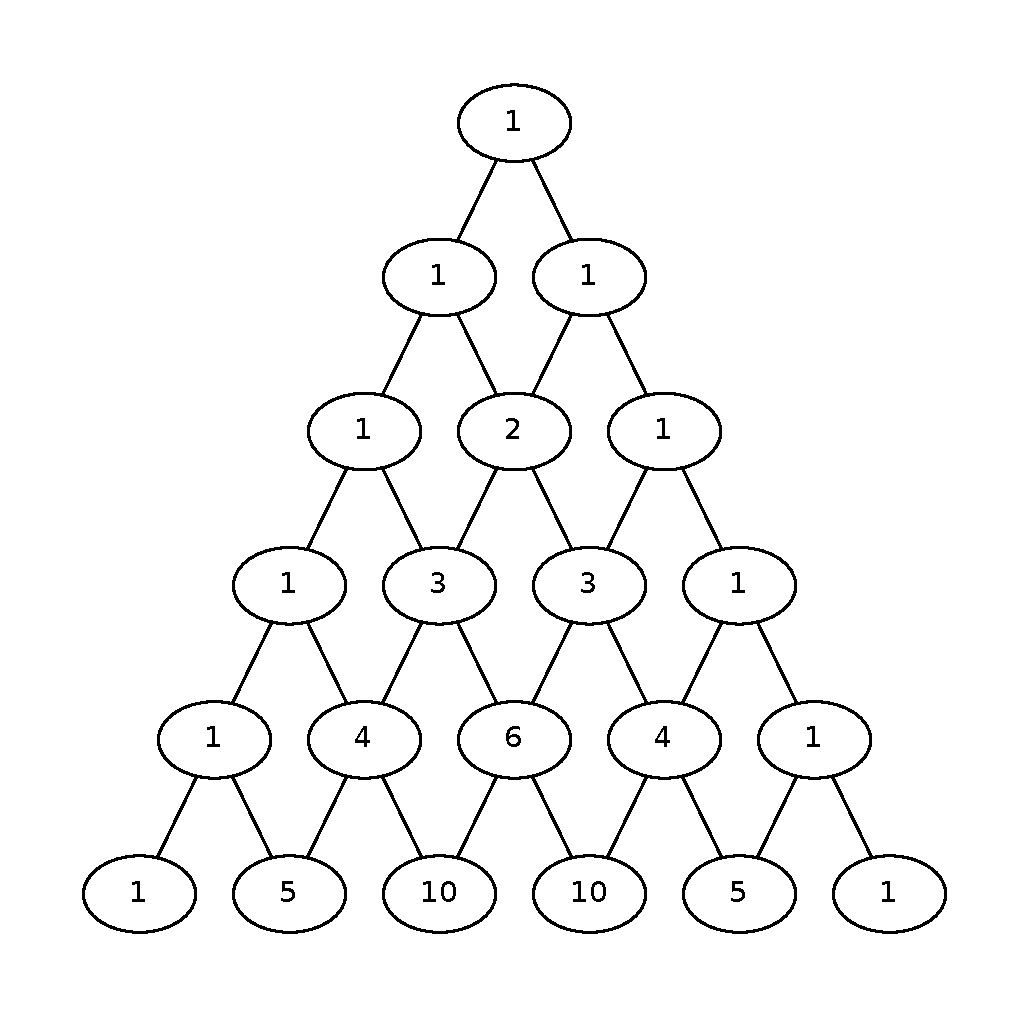
\includegraphics[width=0.6\linewidth]{pascals-triangle.pdf}
\caption{Pascal's triangle. \label{pascals-triangle-fig}}
\end{figure}
\subsubsection{Testing for correctness}
\label{sec-4-1-3}

Now that Pascal's triangle has been constructed and a graphic
representation prepared, it is worth asking whether the triangle
itself is correct.  Because the sum of successive diagonals of the
triangle yields the Fibonacci series, it is possible to verify that
the triangle is correct.  This can be done in many ways; here, it is
done with a short block of \proglang{Emacs Lisp} code that takes a row of numbers
and a number \texttt{n} and returns \texttt{pass} if the sum of the numbers in the
row is equal to the nth Fibonacci number and returns \texttt{fail} otherwise.
Calls to this code block can be embedded into the tabular view of
Pascal's triangle using spreadsheet-style formulas.  When the
spreadsheet is calculated, it returns \texttt{pass} for each of the five
diagonals, confirming that the implementation of Pascal's triangle is
correct.


\begin{Code}
#+source: pst-check
#+begin_src emacs-lisp :var row='(1 2 1) :var n=0 :exports code
  (defun fib (n)
    (if (<= n 2)
        1
      (+ (fib (- n 1)) (fib (- n 2)))))

  (let ((row (if (listp row) row (list row))))
    (if (= (fib n) (reduce #'+ row))
        "pass"
      "fail"))
#+end_src

#+results: pascals-triangle
| 0 |    1 |    2 |    3 |    4 |    5 |
|---+------+------+------+------+------|
|   | pass | pass | pass | pass | pass |
| 1 |      |      |      |      |      |
| 1 |    1 |      |      |      |      |
| 1 |    2 |    1 |      |      |      |
| 1 |    3 |    3 |    1 |      |      |
| 1 |    4 |    6 |    4 |    1 |      |
| 1 |    5 |   10 |   10 |    5 |    1 |
#+TBLFM: @2$2='(sbe pst-check (row @3$1) (n @1$3))
#+TBLFM: @2$3='(sbe pst-check (row @4$1..@4$2) (n @1$4))
#+TBLFM: @2$4='(sbe pst-check (row @5$1..@5$2) (n @1$5))
#+TBLFM: @2$4='(sbe pst-check (row @6$1..@6$2) (n @1$6))
#+TBLFM: @2$4='(sbe pst-check (row @7$1..@7$2) (n @1$7))
\end{Code}
\subsection{Literate programming---cocktail sort}
\label{sec-4-2}

Cocktail sort\footnote{This implementation of Cocktail Sort is adapted
from \href{http://rosettacode.org/}{http://rosettacode.org/}. } is a variation of bubble sort in which
the direction of array traversal is alternated with each pass.  As a
result cocktail sort is more efficient than bubble sort for arrays
with small elements located at the end of the array.

The following literate programming example demonstrates an
implementation of cocktail sort logically divided among three code
blocks.  The code blocks may be \emph{tangled} to produce a single source
code file named \texttt{cocktail.c} which may then be compiled to generate a
command line executable.

The \texttt{cocktail.c} code block uses standard literate programming
syntax.  During tangling code block references
(i.e.,
  \verb=<<block-name>>=
) are expanded to combine the three parts of the program: the standard
\proglang{C} header for input/output in block \texttt{cocktail.c}; the implementation of
the cocktail sort algorithm in block \texttt{cocktail-sort}; and the
command-line mechanism to accept input and return results in block
\texttt{main}.  The \texttt{:noweb yes} header argument enables the expansion of
\pkg{noweb} references and the \texttt{:tangle cocktail.c} header argument
specifies the name of the target source code file.


\begin{Code}
#+source: cocktail.c
#+begin_src C :noweb yes :tangle cocktail.c
  #include <stdio.h>
  <<cocktail-sort>>
  <<main>>
#+end_src
\end{Code}






A standard \proglang{C} language \texttt{main} method is used to collect command line
arguments, call the sorting algorithm on the supplied arguments, and
print the results.


\begin{Code}
#+source: main
#+begin_src C
  int main(int argc, char *argv[]) {
    int lst[argc-1];
    int i;
    for(i=1;i<argc;i++)
      lst[i-1] = atoi(argv[i]);
    sort(lst, argc-1);
    for(i=1;i<argc;i++)
      printf("%d ", lst[i-1]);
    printf("\n");
  }
#+end_src
\end{Code}






In the implementation of cocktail sort the array is repeatedly
traversed in alternating directions, swapping out-of-order elements.
The actual swapping of elements is handled by \texttt{swap}, which sets the
\texttt{swapped} flag when it swaps elements, but leaves the flag alone if
the elements are already in sorted order.  This process continues
until no more swaps have been made and the array is sorted.


\begin{Code}
#+source: cocktail-sort
#+begin_src C :noweb yes
  void sort(int *a, unsigned int l)
  {
    int swapped = 0;
    int i;

    do {
      for(i=0; i < (l-1); i++) {
        <<swap>>
      }
      if ( swapped == 0 ) break;
      swapped = 0;
      for(i= l - 2; i >= 0; i--) {
        <<swap>>
      }
    } while(swapped > 0);
  }
#+end_src
\end{Code}






The \texttt{swap} method performs conditional swapping of adjacent array
elements that are not in sorted order.  It sets the \texttt{swapped} flag if
it performs a swap.


\begin{Code}
#+source: swap
#+begin_src C
  if ( a[i] > a[i+1] ) {
    int temp = a[i];
    a[i] = a[i+1];
    a[i+1] = temp;
    swapped = 1;
  }
#+end_src
\end{Code}






In usual literate programming practice these parts can be tangled out
to the file \texttt{cocktail.c}, as indicated by the \texttt{:tangle} header
argument of the \texttt{cocktail.c} code block.  Alternately the expanded
code block can be compiled and evaluated from within the \pkg{Org-mode} file
using the following \texttt{\#+call} line.  The \texttt{\#+call:} line syntax can be
used to execute code blocks as functions, specifying arguments and
header arguments.  The result of executing the remote code block is
inserted locally, as shown.


\begin{Code}
#+call: cocktail.c[:cmdline 8 7 6 3 2 4 78]()

#+results: cocktail.c[:cmdline 8 7 6 3 2 4 78]()
: 2
: 3
: 4
: 6
: 7
: 8
: 78
\end{Code}
\subsection{Reproducible research---live climate data}
\label{sec-4-3}

By referencing external data, a work of Reproducible Research can
remain up-to-date long after its initial composition and publication.
This example demonstrates the ability of code blocks in an \pkg{Org-mode}
document to reference external data, to construct and use local stores
of data outside the document, and to maintain persistent state in
external sessions, all in an automated fashion. This allows each
reader to recreate the document with up-to-date data, and to
populate a full local workspace with the data used in the document.

This example references climate change data from the US National
Oceanic and Atmospheric Administration (NOAA). The data set is much
larger (hundreds of thousands of rows) than the Pascal's Triangle
example above (Section \ref{pascals-triangle}). Accordingly, this
example demonstrates a different style of working with executable code
blocks in \pkg{Org-mode}: instead of transferring large amounts of data
between blocks via \pkg{Org-mode} tables and \proglang{Emacs Lisp}, we use temporary
plain text files on disk and a dedicated external database. The
example is implemented with command-line tools commonly available on
Unix-like systems, the \proglang{sqlite} database, and \proglang{R}.  These software tools
were chosen to illustrate the use of popular data processing tools
from within \pkg{Org-mode}.  It is worth pointing out, however, that at each
step of the way alternatives exist, one or more of which might
simplify the example for any particular user.

The first two code blocks fetch and parse data from NOAA using
standard command-line tools.



\begin{Code}
#+source: raw-temps
#+headers: :results output :file raw-temps.csv
#+begin_src sh :exports none
  curl ftp://ftp.ncdc.noaa.gov/pub/data/ghcn/v2/v2.mean_adj.Z \
      |gunzip \
      |perl -pe 's/-9999/ NA/g' \
      |perl -pe 's/^([0-9]{3})([0-9]{8})([0-9])/$1 $2 $3 /' \
      |perl -pe 's/ +/,/g'
#+end_src

#+source: country-codes
#+headers: :results output :file country-codes.csv
#+begin_src sh :exports none
  curl ftp://ftp.ncdc.noaa.gov/pub/data/ghcn/v2/v2.slp.country.codes \
      |perl -pe 's/ *$//' \
      |perl -pe 's/ +/,/'
#+end_src
\end{Code}








Next, the output of the first two blocks is used to create a local
database of the combined climate data.  In the case of very large data
sets it may be preferable to use an external store like a database
rather than storing the data as plain text in the \pkg{Org-mode} buffer.


\begin{Code}
#+headers: :var raw-temps-file=raw-temps :var codes-file=country-codes
#+begin_src sqlite :db climate.sqlite :exports none :results silent
  drop table if exists temps;
  create table temps (country,station,replicate,year,jan,feb,
         mar,apr,may,jun,jul,aug,sep,oct,nov,dec);
  drop table if exists countries;
  create table countries (code, name);
  .separator ","
  .import $raw-temps-file temps
  .import $codes-file countries
#+end_src
\end{Code}






The \texttt{R-init} code block reads a subset of the data from the \proglang{sqlite}
database and splits the data into a separate time series for each
weather station, in an ESS \proglang{R} session named \texttt{*R-climate*}. The
variables persist in the \texttt{*R-climate*} session after the code block
exits, so they can be manipulated by other \proglang{R} code blocks that use the
\texttt{*R-climate*} session.


\begin{Code}
#+source: R-init
#+headers: :var dbname="climate.sqlite"
#+begin_src R :session *R-climate* :exports results :results silent
  library("RSQLite")
  con <- dbConnect(dbDriver("SQLite"), dbname=dbname)
  query <- paste("SELECT temps.station, temps.year, temps.jul",
                 "FROM temps, countries",
                 "WHERE countries.code=temps.country",
                 "AND countries.name='UNITED STATES OF AMERICA'",
                 "AND temps.replicate='0'",
                 "ORDER BY year;")
  temps <- dbGetQuery(con, query)
  temps$year <- as.integer(temps$year)
  temps$jul <- as.numeric(temps$jul)/10
  temps.by.station <- split(temps, temps$station, drop=TRUE)
#+end_src
\end{Code}






Finally the persistent variables in the \texttt{*R-climate*} session are used
to generate figures from the climate data. Here we fit a straight line
to the July temperatures at each station which has measurements
spanning the period 1880-1980, and plot a histogram of the fitted
slope parameters. The figure is written to a PDF file for
incorporation into the exported document (Figure
\ref{fig:climate-trend}).


\begin{Code}
#+srcname: R-graph
#+headers: :results graphics :file temp-trends.pdf
#+begin_src R :session *R-climate* :exports results
  include.station <- function(station)
      station$year[1] <= 1880 && station$year[nrow(station)] >= 1980
  fit.slope <- function(station)
      with(station, coefficients(lm(jul ~ year))["year"])
  included <- sapply(temps.by.station, include.station)
  slopes <- sapply(temps.by.station[included], fit.slope)
  hist(slopes)
#+end_src

#+results: R-graph
[[file:temp-trends.pdf]]
\end{Code}






\begin{figure}[t!]
\centering
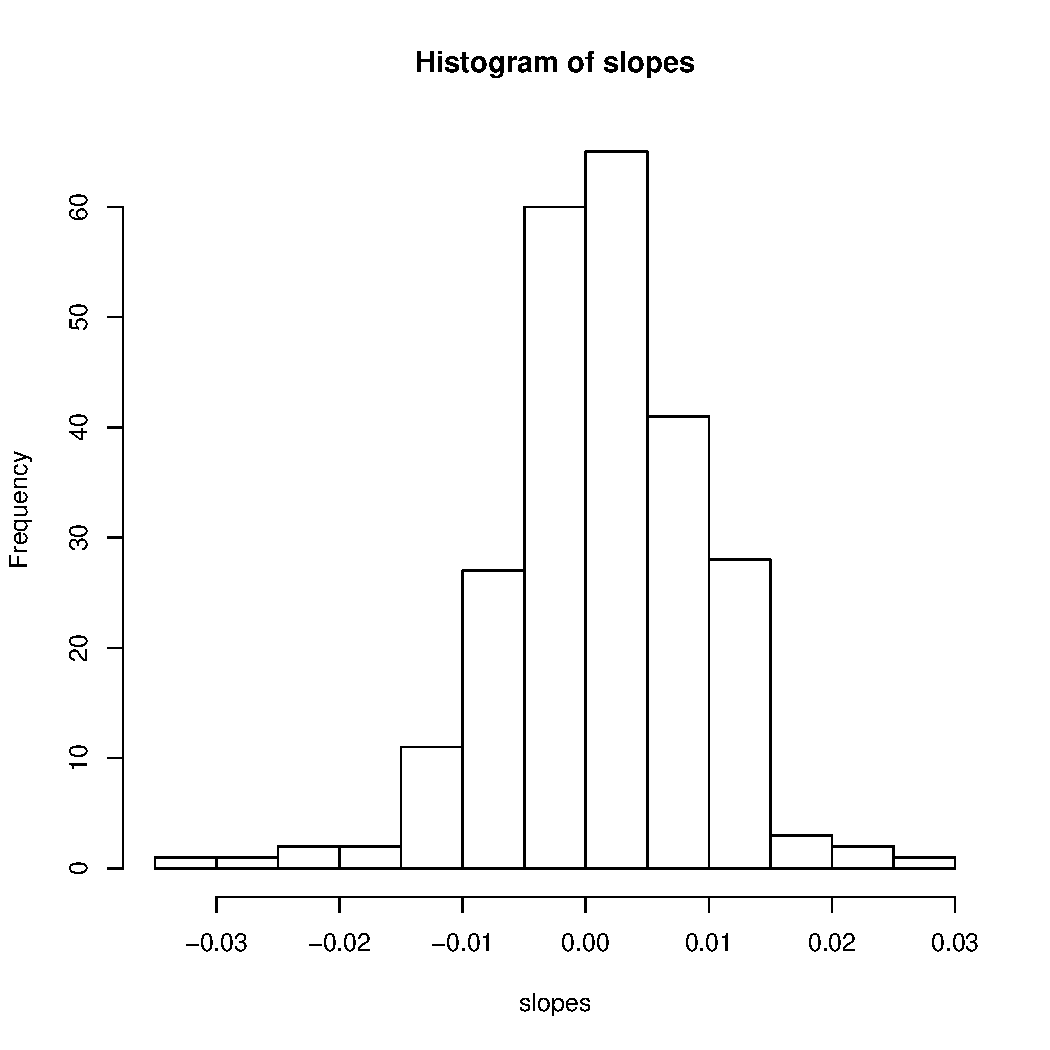
\includegraphics[width=0.7\linewidth]{temp-trends.pdf}
\caption{Temperature trends between 1880 and the present at weather stations in the USA. \label{fig:climate-trend}}
\end{figure}
\section{Discussion}
\label{sec-5}
\label{discussion}


\pkg{Org-mode} has several features that make it a potentially useful tool
for a community of researchers and developers.  These include:

\begin{description}
\item[Open source] \pkg{Org-mode} is open source software.  Its inner
     workings are publicly visible, and its copyright is owned by the
     Free Software Foundation \citep{fsf}.  This ensures that
     \pkg{Org-mode} and any work deriving from \pkg{Org-mode} will always be
     fully open to public scrutiny and modification.  These are
     essential qualities for software tools used for reproducible
     research.  The transparency required for computational results to
     be accepted by the scientific community can only be achieved when
     the workings of each tool in the scientist's tool chain is open to
     inspection and verification.
\item[Widely available] Software used in reproducible research should be
     readily available and easily installed by readers.  \pkg{Org-mode} is
     freely available and, as of the next major release of Emacs
     (version 24), \pkg{Org-mode}, including all of the facilities discussed
     herein, will be included in the Emacs core.  Emacs is one of the
     most widely ported software applications, making possible the
     installation and use of \pkg{Org-mode} on a wide variety of user
     systems.
\item[Active community] The \pkg{Org-mode} community provides ready
     support to both novice users with basic questions and to
     developers seeking to extend \pkg{Org-mode}.  The development of
     \pkg{Org-mode} would not have been possible without the attention and
     effort of this community.
\item[General and extensible] A main design goal of \pkg{Org-mode}'s support
     for working with source code was generality.  As a result, it
     displays no reproducible research or literate programming bias,
     supports arbitrary programming languages, and exports to a wide
     variety of file types, including ASCII, \LaTeX{}, \proglang{HTML}, and DocBook.
     Researchers and software developers who adopt \pkg{Org-mode} can be
     confident that it will be able to adapt to new languages or modes
     of development.
\item[Integration] \pkg{Org-mode} leverages the sophisticated editing modes
     available in Emacs for both natural and computational languages.
\end{description}


Literate programming and reproducible research systems are typically
prescriptive and difficult to use, and this cost of adoption has kept
them from spreading more widely through the computing community.
\pkg{Org-mode} enables users to progress gradually from simple text editing
to sophisticated data processing and code evaluation, thereby lowering
the adoption cost of these techniques.  By consolidating all code,
data, and text of research and development projects, \pkg{Org-mode} increases
the likelihood of their retention.  We believe that with its ease of
adoption, familiar environment, and universal applicability across
programming languages, \pkg{Org-mode} represents a qualitative advance in
literate programming and reproducible research tools.

\pkg{Org-mode} has the potential to advance the expectation that all
computational projects include \emph{both} code and prose; the arguments
that Knuth advanced for literate programming are no less valid today,
and the pervasive use of computational tools in scientific research
makes reproducible research practices essential to the peer review
process.  \pkg{Org-mode} provides researchers and software developers with a
powerful tool to communicate their work and make it more accessible.
\section{Acknowledgments}
\label{sec-6}
\label{acknowledgments}

The authors gratefully acknowledge the \pkg{Org-mode} community whose ideas
and feedback both guided and motivated this work.  Additionally Eric
Schulte would like to acknowledge Counsyl for its support of this
development.

  \bibliography{jss705}

\end{document}
